\section{Implementation details}
\label{app:impl}
\subsection{Preprocessing parameters}
Separator lines on IAM forms are found by a horizontal morphological opening with a 400~px kernel and a row-sum threshold of 30\% of the page width (retried with a 250~px kernel and 15\% for faint lines); the handwritten area lies between the second separator and the ``Name'' footer line, with a fallback to fixed fractions when a line is missing.
CVL pages use a 300~px kernel and a 20\% threshold for the line under the printed source text.
The background is estimated by a $25\times25$ morphological closing followed by a Gaussian blur of $\sigma=20$, and the page is divided by it.
A page is rejected when either side is shorter than 200~px or the aspect ratio exceeds 4, and as blank when the ink fraction (pixels darker than $0.75\times$ the median) is below $0.25\%$.
This threshold was lowered from $0.5\%$ after 34 CVL pages written with thin pens were wrongly marked blank.
Of the Kaggle real-versus-generated set, 2,352 pages were kept; duplicates and strip-shaped images were removed by the hash and geometry filters.

\subsection{Patch sampling}
Candidate windows are centred on a random subset of ink pixels (1,500 draws); a window is kept if its ink fraction reaches the first level of the sequence 5\%, 3\%, 1.5\%, 0.8\% at which at least $K$ windows qualify.
If even 0.8\% fails, windows with at least 0.4\% ink are resampled with replacement, and a page with none is rejected rather than padded.
For evaluation the random generator is seeded from a hash of the page path, so the same patches are used in every evaluation; the demonstration seeds it from a hash of the normalised image instead.

\subsection{Training procedure}
Training uses mixed precision, gradient clipping at 1.0, an exponential moving average of the weights (decay 0.999) for validation and testing, and validation every second epoch.
The training loop recovers from out-of-memory errors by halving the number of patches (down to 8), skips non-finite losses, and writes checkpoints safely on termination signals, so an interrupted run can resume; a resumed run refuses a checkpoint from a different seed.
Content-matched CVL batches pick two texts that enough writers have written and use only those writers; the nearest-neighbour batches use centroids recomputed every 10 epochs.
A label-shuffle control (writer labels permuted inside each batch) keeps the loss at $\ln 24=3.135$, confirming that no information leaks through page order or file names.

\subsection{Compute}
\begin{table}[t]
\caption{Measured compute on the RTX 4050 laptop GPU (6~GB).}
\label{tab:compute}
\centering\scriptsize
\begin{tabular}{ll}
\toprule
Item & Value \\
\midrule
GPU memory in training & about 3.5~GB \\
Time per epoch (70 steps, with distillation) & 25 to 28~s \\
Main run (three seeds) & about 50 min of training each \\
Ablation run (40 epochs) & about 20 min each \\
Reported runs in total & about 5 GPU hours \\
Demonstration inference & CPU only, about 2 to 3~s per comparison \\
\bottomrule
\end{tabular}
\end{table}

\section{Complete multi-reference results}
\label{app:multiref}
\Cref{tab:mrfull} gives every fusion rule at every number of references on the fixed writer sets used in \Cref{fig:multiref}, and \Cref{tab:mrn5} the smaller set of IAM writers with at least six pages that allows five references.
All entries are test EER (\%), mean $\pm$ standard deviation over three seeds; the sets use nested references and the same impostor queries for every $N$.
The maximum rule is lowest at $N=2$ on IAM and at $N=2,3$ on CVL, and the centroid is lowest at $N=3$ on IAM.
Differences between rules are of the order of the seed spread on IAM, so the choice of rule matters mainly on CVL.

\begin{table}[t]
\caption{Test EER (\%) for every fusion rule and number of references, on one fixed writer set per corpus.}
\label{tab:mrfull}
\centering\scriptsize
\setlength{\tabcolsep}{3pt}
\resizebox{\columnwidth}{!}{\begin{tabular}{llccc}
\toprule
Corpus (writers) & Rule & $N{=}1$ & $N{=}2$ & $N{=}3$ \\
\midrule
IAM (45) & mean & 2.25$\pm$0.05 & 1.79$\pm$0.19 & 1.59$\pm$0.21 \\
IAM (45) & max & 2.25$\pm$0.05 & 1.37$\pm$0.09 & 1.44$\pm$0.11 \\
IAM (45) & top-2 & 2.25$\pm$0.05 & 1.79$\pm$0.19 & 1.48$\pm$0.09 \\
IAM (45) & centroid & 2.25$\pm$0.05 & 1.57$\pm$0.11 & 1.22$\pm$0.12 \\
\midrule
CVL (62) & mean & 6.76$\pm$0.38 & 7.01$\pm$0.63 & 5.99$\pm$0.71 \\
CVL (62) & max & 6.76$\pm$0.38 & 4.68$\pm$0.44 & 3.31$\pm$0.20 \\
CVL (62) & top-2 & 6.76$\pm$0.38 & 7.01$\pm$0.63 & 5.13$\pm$0.18 \\
CVL (62) & centroid & 6.76$\pm$0.38 & 5.22$\pm$0.54 & 5.19$\pm$0.73 \\
\bottomrule
\end{tabular}
}
\end{table}

\begin{table}[t]
\caption{Test EER (\%) on the 17 IAM writers with at least six pages, which allows $N=5$.}
\label{tab:mrn5}
\centering\scriptsize
\setlength{\tabcolsep}{3pt}
\resizebox{\columnwidth}{!}{\begin{tabular}{lcccc}
\toprule
IAM, 17 writers with $\geq$6 pages & $N{=}1$ & $N{=}2$ & $N{=}3$ & $N{=}5$ \\
\midrule
mean & 1.99$\pm$0.32 & 1.42$\pm$0.33 & 1.18$\pm$0.06 & 0.93$\pm$0.23 \\
max & 1.99$\pm$0.32 & 1.13$\pm$0.03 & 1.18$\pm$0.10 & 1.13$\pm$0.33 \\
top-2 & 1.99$\pm$0.32 & 1.42$\pm$0.33 & 1.13$\pm$0.23 & 0.83$\pm$0.19 \\
centroid & 1.96$\pm$0.31 & 1.32$\pm$0.06 & 1.08$\pm$0.30 & 0.81$\pm$0.22 \\
\bottomrule
\end{tabular}
}
\end{table}

\section{Thresholds and calibration per seed}
\label{app:calib}
\Cref{tab:calib} lists, for each seed, the verdict thresholds fixed on validation trials (three references, centroid rule) and the expected calibration error of the raw score and of the two calibrators.
For IAM the two thresholds coincide because the corpus is separable on validation (\Cref{sec:results}).
Thresholds differ by up to 0.06 between seeds on CVL, so a deployed system would have to be calibrated for its own model and data.

\begin{table}[t]
\caption{Verdict thresholds (cosine) and expected calibration error per seed.}
\label{tab:calib}
\centering\scriptsize
\setlength{\tabcolsep}{2.5pt}
\resizebox{\columnwidth}{!}{\begin{tabular}{llccccc}
\toprule
Corpus & Seed & $\tau_{\mathrm{lo}}$ & $\tau_{\mathrm{hi}}$ & ECE raw & ECE Platt & ECE isotonic \\
\midrule
IAM & 0 & 0.888 & 0.888 & 0.213 & 0.066 & 0.010 \\
IAM & 1 & 0.884 & 0.884 & 0.218 & 0.066 & 0.009 \\
IAM & 2 & 0.898 & 0.898 & 0.222 & 0.078 & 0.008 \\
\midrule
CVL & 0 & 0.824 & 0.909 & 0.229 & 0.091 & 0.027 \\
CVL & 1 & 0.780 & 0.888 & 0.220 & 0.074 & 0.024 \\
CVL & 2 & 0.698 & 0.846 & 0.201 & 0.064 & 0.010 \\
\bottomrule
\end{tabular}
}
\end{table}

\section{Additional figures}
\label{app:figs}
\begin{figure}[t]
\centering
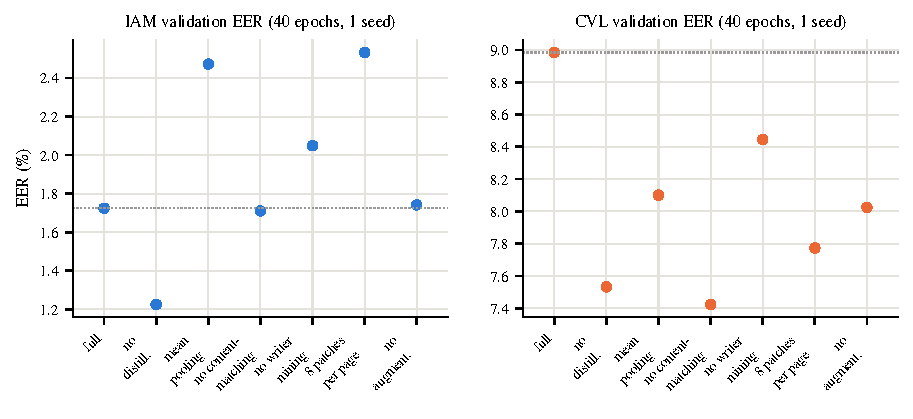
\includegraphics[width=\columnwidth]{figures/fig_ablation}
\caption{Validation EER of the ablation variants (40 epochs, one seed each); the dotted line is the full model.}
\label{fig:abl}
\end{figure}

\begin{figure}[t]
\centering
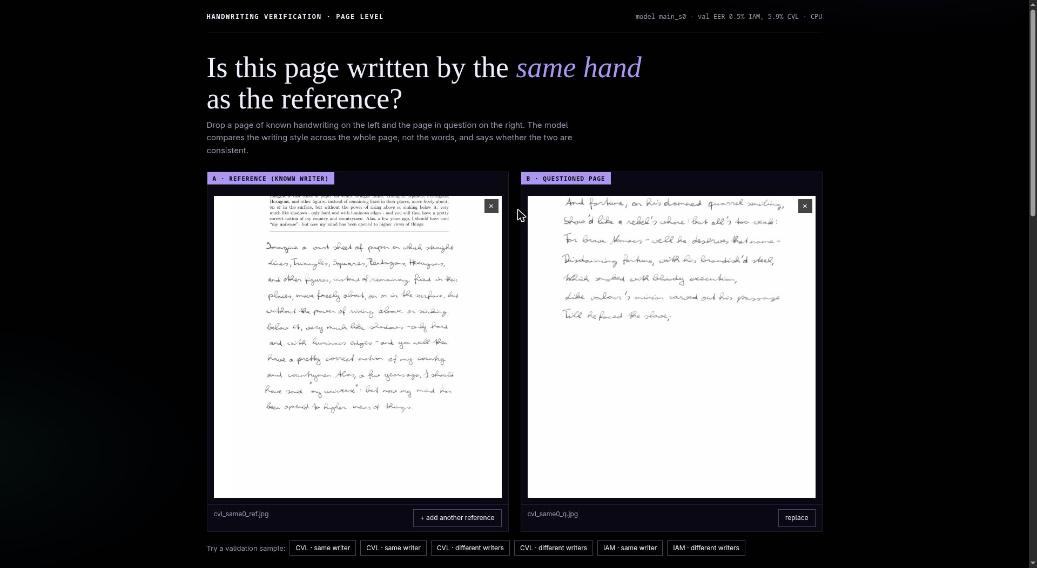
\includegraphics[width=\columnwidth]{figures/demo_inputs.jpg}
\caption{Demonstration service: the reference page and the questioned page are uploaded or chosen from validation samples.}
\label{fig:demo1}
\end{figure}

\begin{figure}[t]
\centering
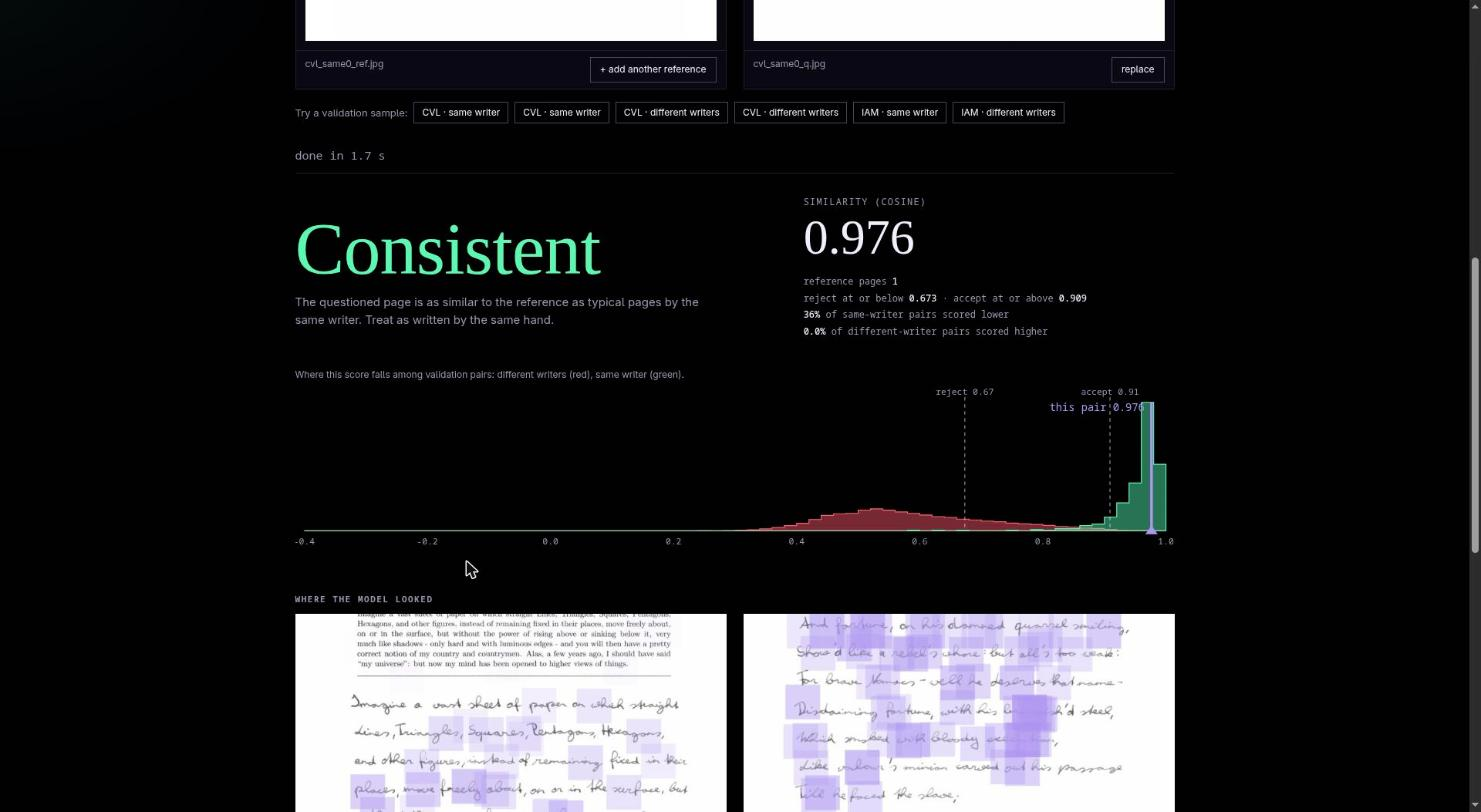
\includegraphics[width=\columnwidth]{figures/demo_result.jpg}
\caption{Demonstration result: verdict, similarity score, position of the score among validation pairs of different writers (red) and the same writer (green), and attention heatmaps.}
\label{fig:demo2}
\end{figure}

\section{Responsible use}
\label{app:ethics}
A verdict of \emph{likely forged} can damage a person, so the system is meant as decision support for a human examiner, not as evidence on its own.
Three properties make caution necessary.
First, the model measures similarity of writing style; a writer who changes style on purpose is rejected (\Cref{tab:fm}), and a skilled imitator has not been tested.
Second, the error rate at a strict operating point is high on content-matched pairs (\Cref{sec:results}), so a single page pair is weak evidence.
Third, thresholds are fitted on validation data of two corpora and may not hold for other paper, pens or scanners; phone photographs differ from the training scans.
The demonstration therefore prints these limits next to every result and returns \emph{inconclusive} when the score lies between the two thresholds.
All pages and models stay on the local machine; the demonstration does not store uploads.
Datasets were used under their own licences, and the IAM copy used here is third-party, so official registration is needed before the data are cited in a submission.

\section{Reproducibility checklist}
\label{app:repro}
\begin{table}[t]
\caption{Where each part of the study lives in the project repository.}
\label{tab:repo}
\centering\scriptsize
\setlength{\tabcolsep}{3pt}
\resizebox{\columnwidth}{!}{%
\begin{tabular}{ll}
\toprule
Part & Module \\
\midrule
Page cache, splits, leakage checks & \texttt{prep\_cache.py}, \texttt{manifests.py} \\
Patch sampler, content-matched batches & \texttt{data.py} \\
Encoder, losses & \texttt{model.py} \\
Training with resume and recovery & \texttt{train.py}, \texttt{run\_train.sh} \\
Baselines & \texttt{baselines.py} \\
Single-reference evaluation, Firemaker, synthetic pages & \texttt{eval.py} \\
Controlled multi-reference study & \texttt{multiref.py} \\
Verdict from saved scores & \texttt{verdict.py} \\
Attention maps and deletion test & \texttt{explain.py} \\
All tables, figures and the abstract & \texttt{report.py} \\
\bottomrule
\end{tabular}}
\end{table}
Each run stores its configuration, per-epoch log and result files; the three seeds are 0, 1 and 2, and all splits use seed 42.
The test sets and Firemaker were evaluated once per seed after training ended, and the two analysis errors found afterwards (overlapping verdict thresholds and a writer set that shrank with $N$) were corrected without retraining and are documented in the repository.
Every number in this paper is generated from the stored result files and listed with its source in a claim-to-evidence map, and the commands to repeat the experiments on GPU and CPU are in the repository documentation.
